\chapter{Optical Enhancement of Core-Shell Nanowire} \label{data}

Given that the profound enhancement of optoeletronic properties of nanowires is
the major theme of this dissertation, it is dutiful to first summarize the
major experimental charateristics of Core-Shell nanowires (CSNWs)

Electron systems in lower dimensions are adequately treated through
perturbation methods. For 1D electron systems (1DES) the correlations among
electrons are much more significant due to higher degrees of confinement. The
electron can either be moving to the left or right and any small or localized
interaction can cause a collective response from the whole system. This is the
condition of broken symmetry, in which the overall status of the system has to
be reformulated. For a 2DES, a broken symmetry occurs at very low densityies of
fermions, in which formation of a Wigner lattice is expected, which is due to
the Coulombic interactions of electrons. Intererstingly for a 1DES, the
direction of movement for fermions is restricted to the left or right.
Consequently, the density of the sytem becomes irrelevant with respect to the
determination of the status of the system. Such a 1D many electron system is
often called a $L\ddot{u}finger$ Liquid, as he was the first person who
successfully formulated these systems.

Importantly, a 1DES can experimentally be realized in various material systems.
These include carbon nanotubes, electrons at the edges of a 2DES, and in
nanowires.

A core-shell nanowire (CSNW) is a quasi-one dimensional structure with a wide
band gap materials, such as AlGaAs, wrapping around a low band gap
semiconductor, such as GaAs.

It is expected that the lower dimensionality in CSNW to have a significant
influence on both optical and electrical properties of the structure. Fot
instantce,

Electrically it is important account for the electron correlations in order to
determine the behavior of the structure. The significant values ofr exchange
and correlation energies in 1DES. makes them an interesting candidate for
probing ther energy dynamics. This, however, imposes various experimental
challenges and theoretical considerations and are deferred to future
investigations.

\section{Growth of Nanowires}

Freestanding quasi-one-dimensional semiconductor nanostructures (nanowires)
based on III-V compound semiconductors, owing to their unique physical
properties, are considered ideal building blocks for the realization of
photonic and electronic nanodevices.

Currently, two bottom-up approaches to the fabrication of freestanding
nanowires are considered: (i) selective area epitaxy
(SAE)~\cite{motohisa2004catalyst} and (ii) metal-catalyst assisted grouth
through the so-called vapor-liquid-solid (VLS) mechanism~\cite{wagner1964vapor,
givargizov1975fundamental}. The latter method relies on the alloying of a metal
catalyst (usually Au) nanoparticle with the semiconductor constituent elements,
supplied through a vapor phse. The as-formed alloy acts as an initial
nucleation site for the material and further guides the nanowire growth, the
diameter of the nanowire being controlled by that of the metal nanoparticle.

An advantage of the VLS method over SAE is that it does not require
nanolithograpic processing of the substrate; furthermore, it is compatible with
most advanced epitaxial grouth techniques for III-V compounds, such as
molecular beam epitaxy, chemical beam epitaxy, and metalorganic vapor phase
epitaxy (MOVPE). 

GaAs nanowires were grwon by low (50mbar) pressure MOVPE using an Aixtron
reactor model AIX200 RD. TMGa and TBAs were used as gallium and arsenic
precursors, respectively. Au nanoparticle deposited on
$(\bar{1}\bar{1}\bar{1})B$ GaAs were used to catalyze the nanowire growth. To
this purpose, VGF-grown semi-insulating (undoped) GaAs wafers oriented
$(\bar{1}\bar{1}\bar{1})B$ were used. The substrates were then first degreased
in isopropanol vapors, etched in $4H_2SO_4:1H_2O_2:2H_2O$ solution for 8 min at
around $40\,^{\circ}\mathrm{c}$, ringsed in de-ionized water and finally dried
under pure $N_2$. Au nanoparticles with \~60 nm diameters were prepared by
reaction of $HAuCl_4$ with sodium citrate in aqueous solution and randomly
deposited on the as-prepared GaAs surface by dropping a small amount of
colloidal solution onto the substrate. The solvent (water) was then evaporated
by holding the samples on a hot plate (in air) or a few minutes; Au
nanoparticle surface densities thus achieved ranged around (1-4). 

After loading the sample into the reactor chamber, its temperature was raised,
and sample annealing was then performed for 10 min to absorb GaAs surface
oxides and organic residules originating from the Au nanoparticle synthesis.
This annealing step would also allow the initial uptake of Ga atoms from the
GaAs substrate into the Au nanoparticles. 

\section{Scanning Electron Microscopy Images} 

Figure 1a is top view SEM image of nanowires of ~100nm diameter core of GaAs,
and ~40nm thick AlGaAs, with the inset showing a magnified image that
demonstrates the rather sparse distribution of the wires. Figure 1b shows the
reflectivity of a GaAs wafer on which 50nm thin film of AlGaAs is grown, and
compares this to the reflectivity spectrum of a Si substrate. As expected,
about 30\% to 55\% of a normally incident light is reflected in bulk Si and GaAs,
with a sharp change for wavelengths near their respective band gaps. Figure 1c
contrasts this with the measured absorption spectrum of two types of GaAs core,
AlGaAs shell (CS) nanowires (BW): those grown on a GaAs substrate (black), and
the others heteroepitaxially grown on a Si substrate (red). The spectra show
that both cases have the signature change of reflectivity at bandgap of GaAs,
i.e., these are due to the GaAs/AlGaAs CSNWs, not the substrate. Importantly,
for the wavelength range of 700-1200nm these core-shells which only occupy ~15%
of the volume compared to thin films of the same height, reflect 2-4\% of light
for the CSNWs grown on Si, and 3-7\% of light for those grown on GaAs substrate.
The beam-width of the incident light being ~1μm, this shows that only a few NWs
are interrogated by light and, normalized to volume, these wires absorb more
than two orders of magnitude more light than their thin-film counterparts.

\begin{figure}
  \caption{Scanning Electron Microscopy image of as-grown GaAs/AlGaAs core-shell nanowires on Sitaken at different magnifications and view angles}
  \centering
  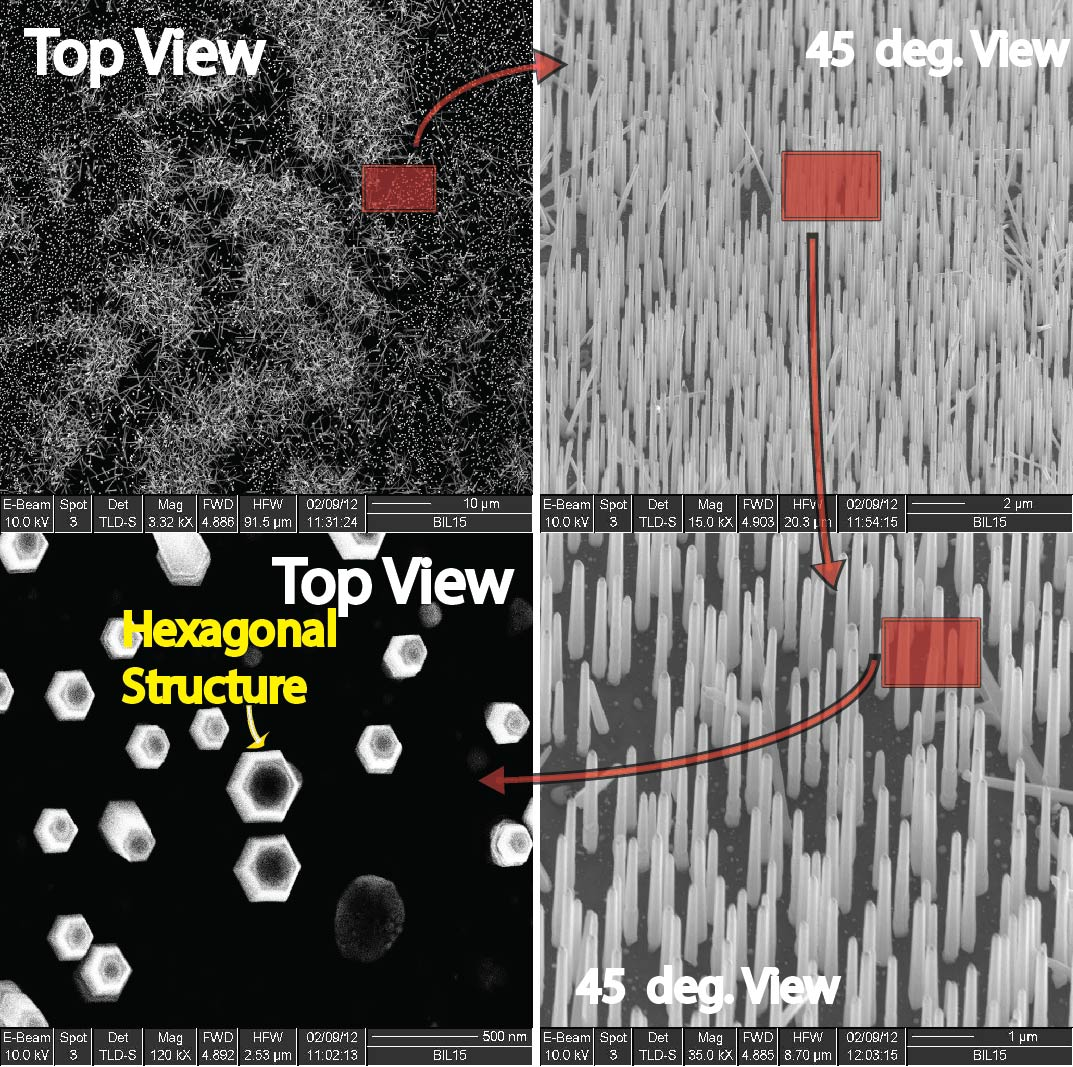
\includegraphics[width=\textwidth]{pictures/Data/SEMNW}
  \label{SEMNW}
\end{figure}

\section{Electrical Characterization of Nanowire}

\begin{figure}
  \caption{Current versus Voltage Measurment under illumination of Core-Shell Nanowire Grown on Si}
  \centering
  \includegraphics[width=\textwidth]{pictures/Data/CSNWIV_light}
  \label{CSNWIV_light}
\end{figure}

\section{Absorption Enhancement} \label{X-ray}

\begin{figure}
  \caption{Reflective Measurement for Bulk GaAs and Si}
  \centering
  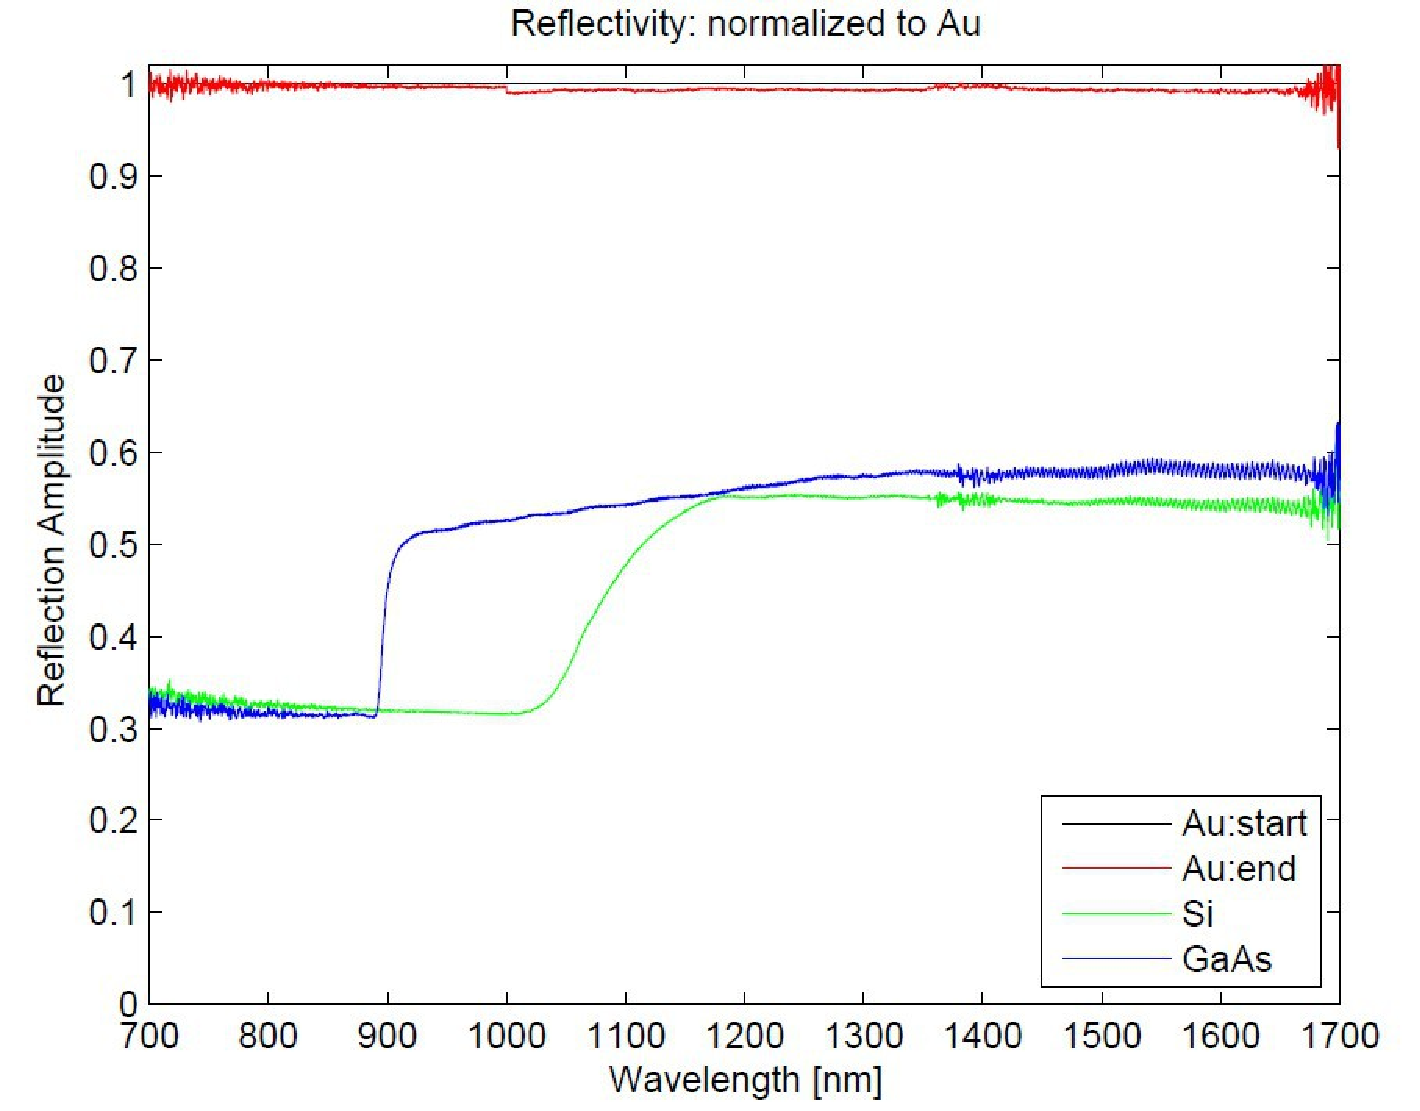
\includegraphics[width=\textwidth]{pictures/Data/reflecbulk}
  \label{reflecbulk}
\end{figure}

\begin{figure}
  \caption{Reflective Measurement for Core-Shell Nanowires Grown on Bulk GaAs and Si}
  \centering
  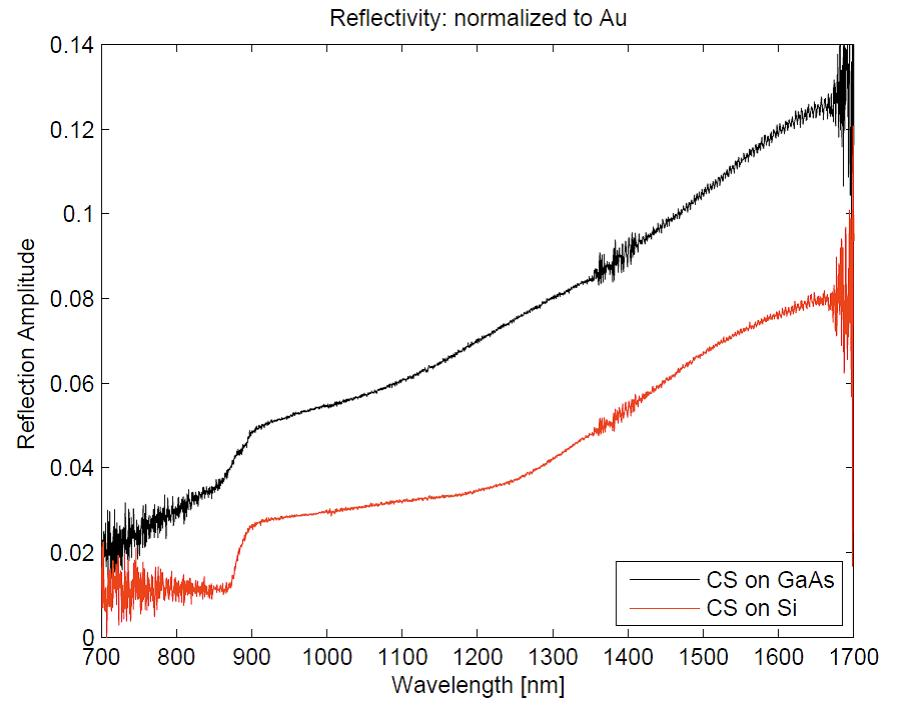
\includegraphics[width=\textwidth]{pictures/Data/reflectCSNW}
  \label{reflectCSNW}
\end{figure}

\section{Emission Enhancement} \label{Dust_data}

\begin{figure}
  \caption{Photoluminescence Experiment for Core-Shell Nanowires Grown on Bulk GaAs and Si}
  \centering
  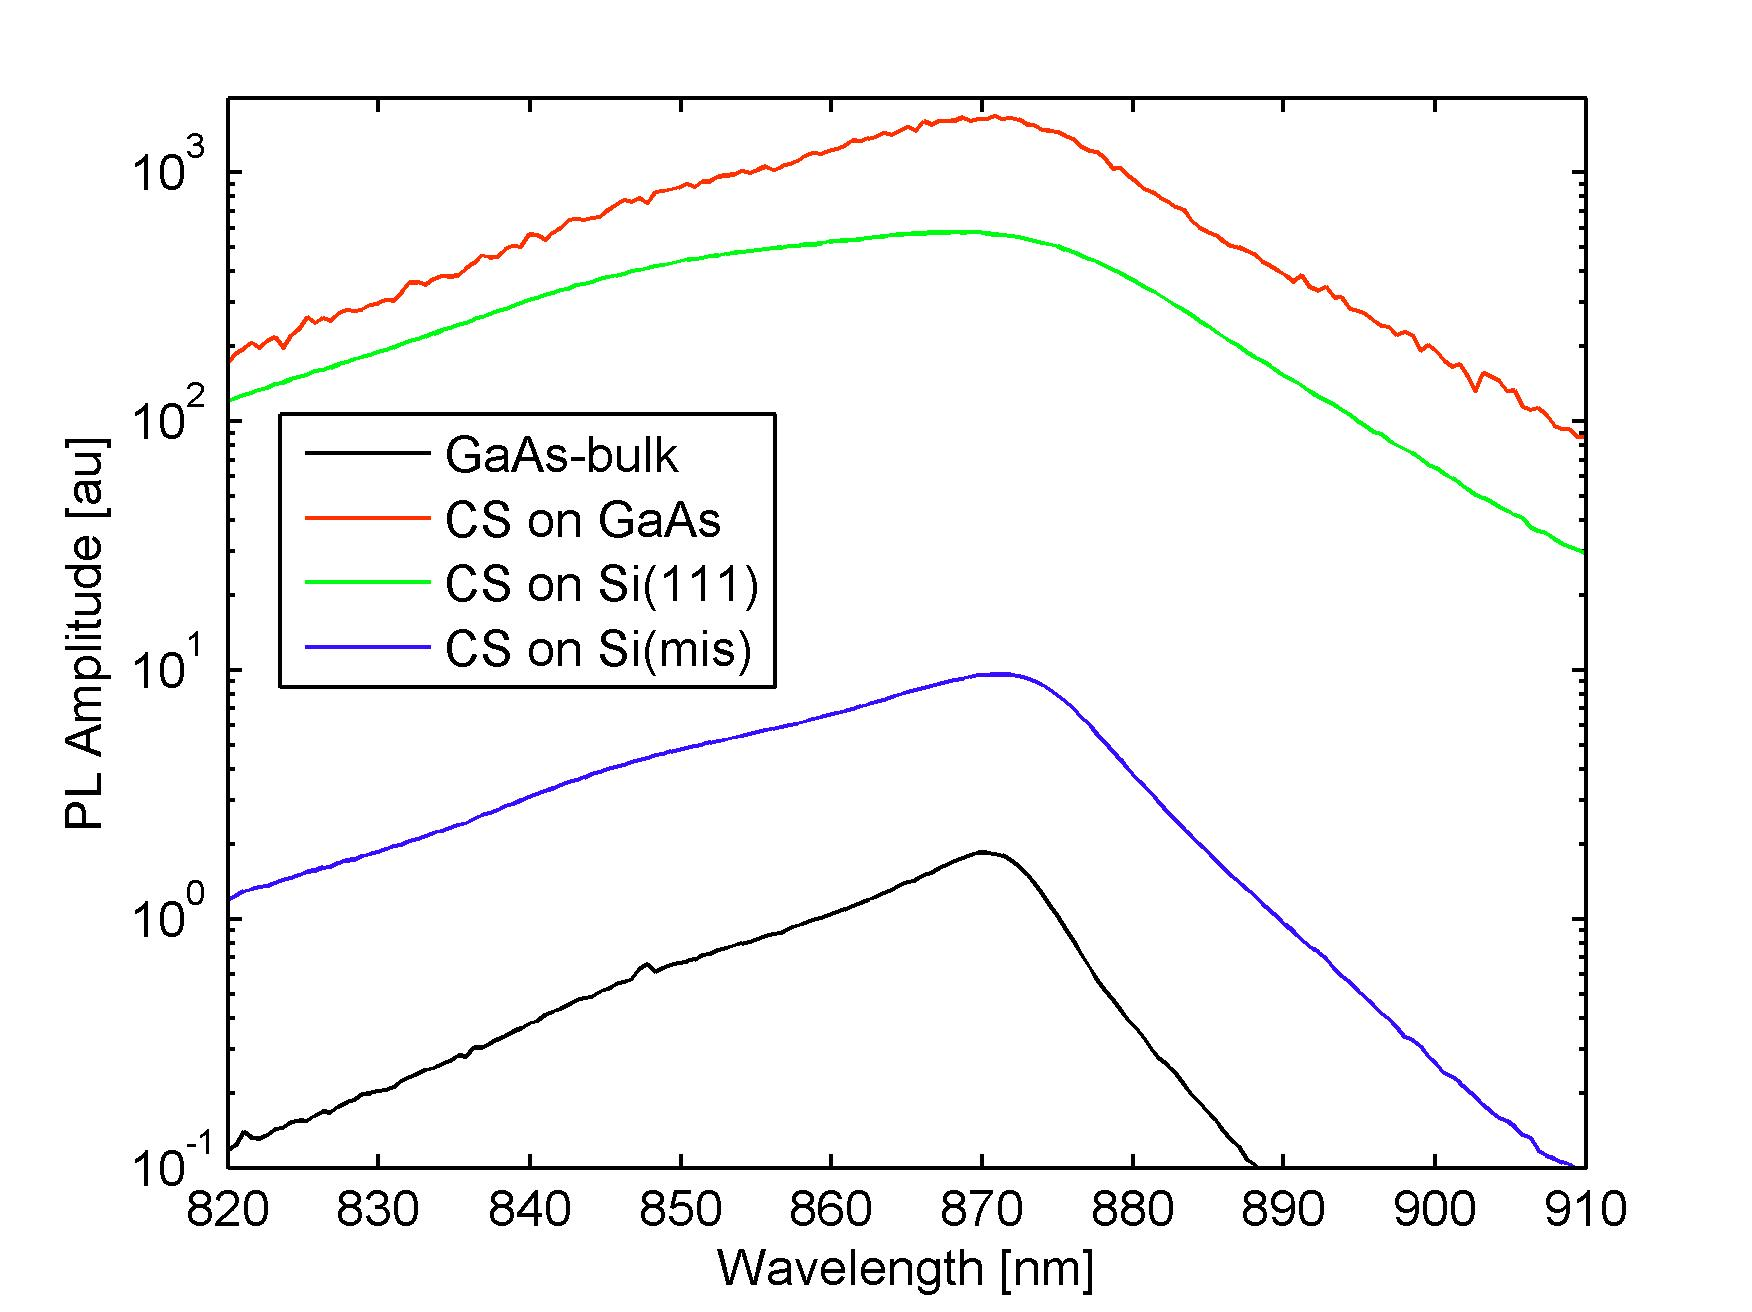
\includegraphics[width=\textwidth]{pictures/Data/PL}
  \label{PL}
\end{figure}

\section{Lasing} \label{BH_data}

Photoluminescence (PL) of bulk GaAs to nanowires grown on GaAs, and on two
directions of Si showed that normalized to the fraction of the volume that
these wires occupy, nealy 10,000 times more brightness is observed in these
wires compared to hin-film. In the case of stimulated emission of light, the
photon mode density $(1+u_\varepsilon)$ plays a crucial role. Figure ~\cite{}
is the photoluminescence (PL) spectrum at various optical pump intensities. As
the excitation laser power increase beyond $5{\mu}W$ a sudden and highly
nonlinear increase in the emission intensity is observed, with pronounced peaks
emerging from 800nm to 850nm that rapidly grows to become several orders of
magnitude stronger than the background emission. The laser amplitude vs.
excitation power demonstrates a threshold of around $5{\mu}W$, followed by
saturation near $12{\mu}W$. The sharp peak has a full width half maximum
(FWHM) that varies from 1.5 to 3.5 nm. This remarkable behavior is achieved in
the as-grown wires with no vertical structure.

\begin{figure}
  \caption{Micro-Photoluminescence measurements with fs-pulsed, 532-nm laser excitation at 250kHz repetition rate shows lasing of the as-grown wires.}
  \centering
  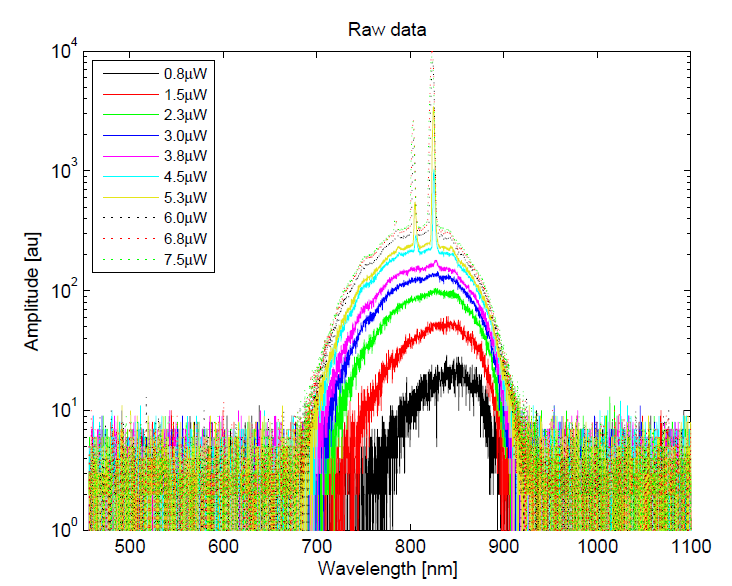
\includegraphics[width=\textwidth]{pictures/Data/lasing}
  \label{lasing}
\end{figure}
